\subsection{Dataset}

\subsection{Baselines}
We compare our algorithm with two kinds of baselines. The first one is methods without leveraging any prior knowledge (no transfer baselines). The second consists of some methods with transfer techniques. Here are the no transfer baselines 

\textbf{0+T(arget):}

\textbf{S(ource)+T(arget):} Only in good oracle.

\textbf{S(ource)+T:}

Transfer baselines:

\textbf{MKTL \cite{jie2011multiclass}:} 

\textbf{Multi-KT \cite{tommasi2014learning}:}

\textbf{MULTIpLE \cite{kuzborskij2013n}:}

\subsection{transfer from good oracle}
\begin{figure*}
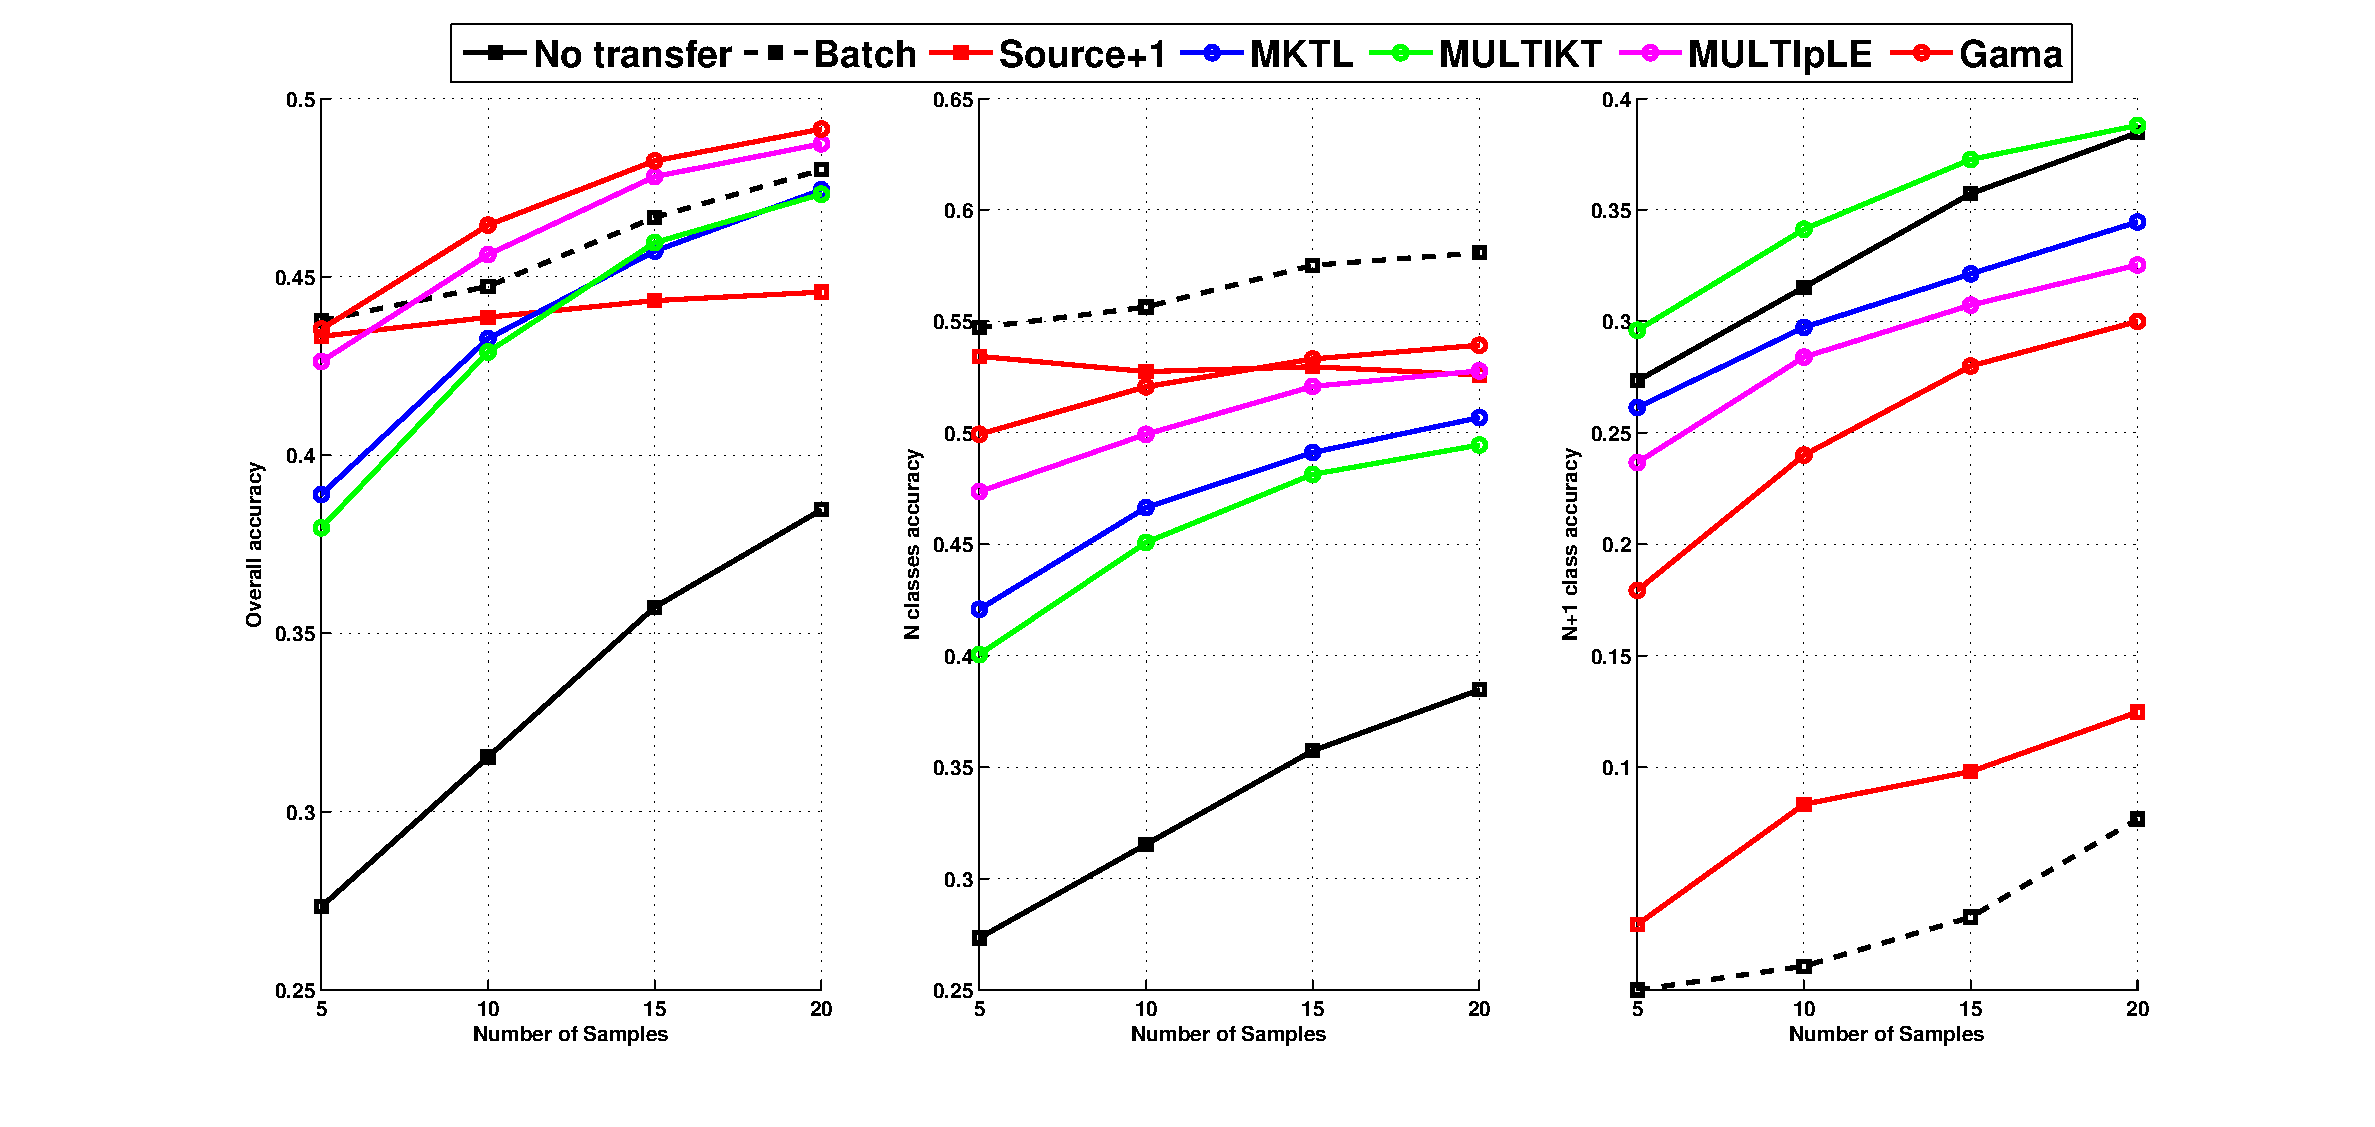
\includegraphics[width=\textwidth,height=5cm]{fig/C2C_RBF.eps}
\caption{Acc for good oracle}
\end{figure*}

\subsection{from bad oracle}
\begin{figure*}
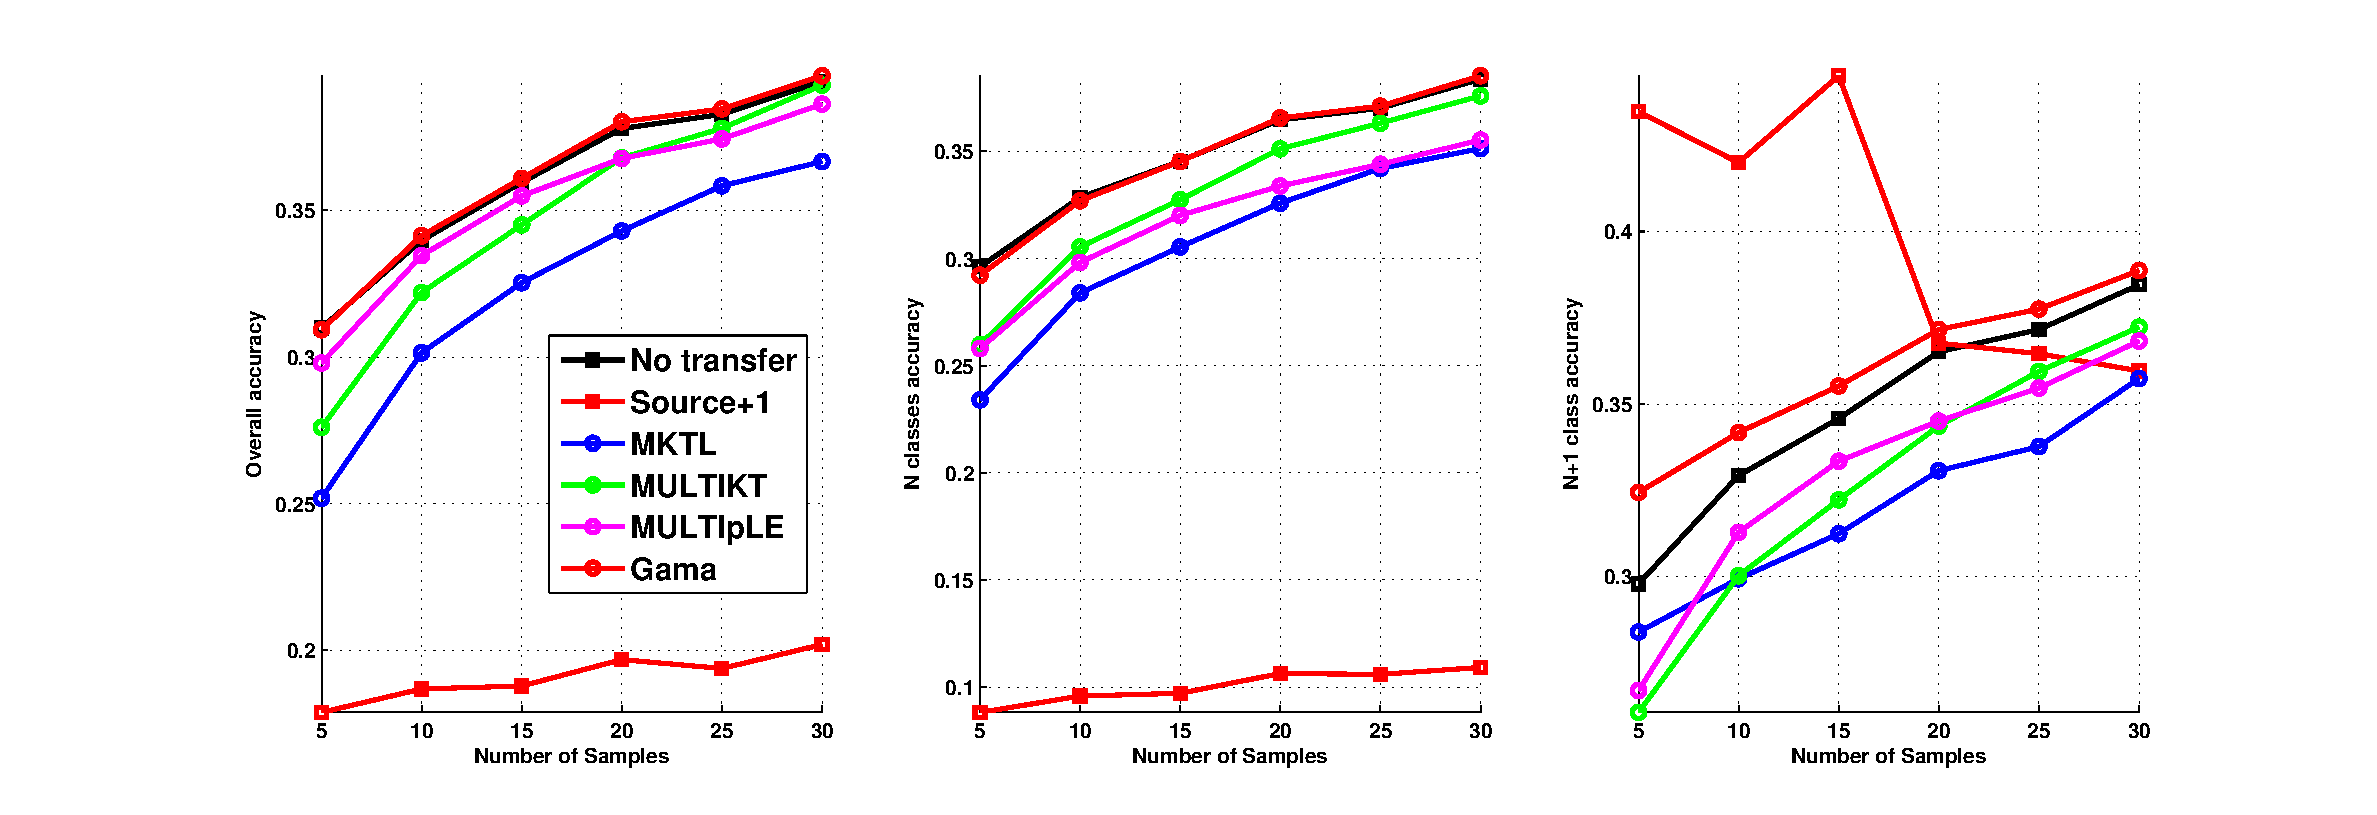
\includegraphics[width=\textwidth,height=5cm]{fig/A2C_RBF_PHOG.eps}
\caption{Acc for bad oracle}
\end{figure*}

\subsection{mixed}

